\chapter{Modelli predittivi utilizzati}
\section{Algoritmi utilizzati per la creazione dei modelli predittivi}
\subsection{Random forest}
Da [https://www.ibm.com/topics/random-forest#:~:text=Random%20forest%20is%20a%20commonly,both%20classification%20and%20regression%20problems.]

\begin{figure}
    \begin{center}    
        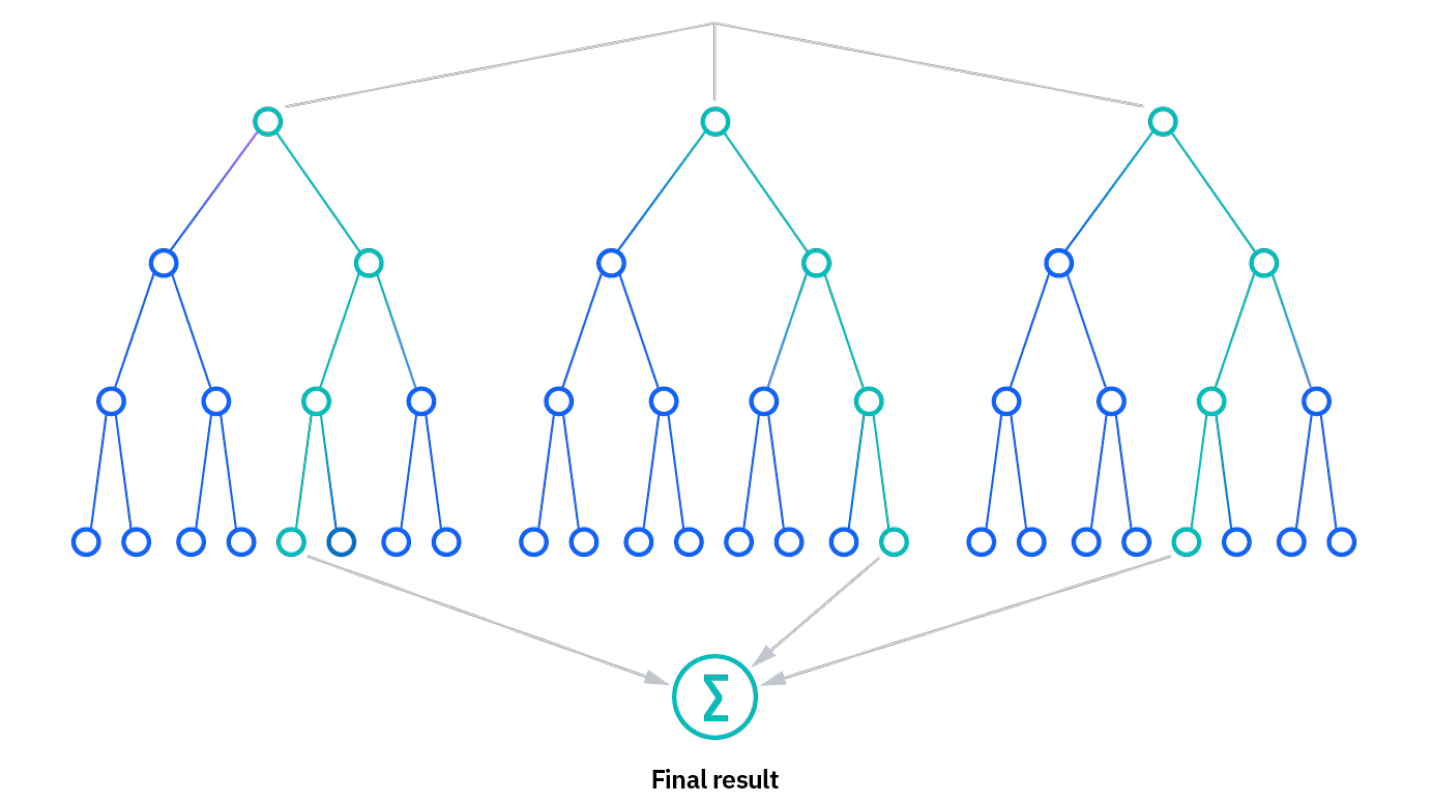
\includegraphics[width=0.9\linewidth]{images/image10.png}
    \end{center}
\end{figure}

La random forest è un algoritmo di apprendimento automatico creato da Leo Breiman e Adele Cutler, che combina l'output di più alberi decisionali col fine di raggiungere un singolo risultato. 

La sua predisposizione intuitiva e la sua flessibilità hanno nutrito l’aumento della sua adozione, in quanto gestisce sia problemi di classificazione che di regressione.

\subsubsection{Alberi decisionali}
Dato che il modello di random forest è composto da più alberi decisionali, è utile descrivere brevemente l'algoritmo dell'albero decisionale. 

Gli alberi decisionali partono da una domanda di base, ad esempio "Dovrei fare surf?". 

A partire da ciò è possibile porre una serie di domande per determinare una risposta, come "C'è un'onda di lungo periodo?" o "Il vento soffia a riva?". 

Queste domande costituiscono i nodi decisionali dell'albero, agendo come mezzo di ripartizione dei dati.

Ogni domanda aiuta l’albero a giungere a una decisione finale, indicata dal nodo foglia raggiunto. 

Le osservazioni che soddisfano i criteri seguiranno il ramo "Sì", mentre quelle che non li soddisfano seguiranno il percorso alternativo. 

Gli alberi decisionali cercano di trovare la miglior suddivisione per i dati, e vengono tipicamente addestrati attraverso l'algoritmo Classification and Regression Tree (CART). 

Metriche come l'impurità di Gini, il guadagno di informazione o l'errore quadratico medio (MSE) possono essere utilizzati per valutare la qualità della suddivisione.

Sebbene gli alberi decisionali siano comuni algoritmi di apprendimento supervisionato, possono essere soggetti a problemi come il bias e l'overfitting. 

Tuttavia, quando più alberi decisionali formano un insieme nell'algoritmo di random forest, predicono risultati più accurati, in particolar modo quando i singoli alberi non sono correlati tra loro.

\subsubsection{L'algoritmo della random forest}
L'algoritmo della random forest è un'estensione del metodo di bagging, in quanto utilizza sia il bagging che la casualità delle features per creare una foresta di alberi decisionali non correlati. 

La casualità delle features, altrimenti nota come bagging delle caratteristiche o "metodo del sottospazio casuale", genera un sottoinsieme casuale di caratteristiche che assicura una bassa correlazione tra gli alberi decisionali. 

Questa è una differenza chiave tra gli alberi decisionali e le random forest, poiché mentre gli alberi decisionali considerano tutte le possibili suddivisioni delle caratteristiche, le random forest selezionano solo un sottoinsieme di quelle caratteristiche.

Tornando all'esempio "dovrei fare surf?", le domande che potrei porre per determinare la previsione potrebbero non essere così esaustive come il set di domande di un altro utente. 

Tenendo conto di tutta la potenziale variabilità dei dati, possiamo ridurre il rischio di overfitting, di bias e di varianza complessiva, ottenendo previsioni via via più precise.

\subsubsection{Come funziona}
Gli algoritmi delle random forest hanno tre iperparametri principali da impostare prima dell'allenamento. 
Questi includono: 

\begin{itemize}
  \item la dimensione del nodo, 
  \item il numero di alberi, 
  \item il numero di caratteristiche campionate
\end{itemize}

Da lì, il classificatore della random forest può essere utilizzato per risolvere problemi di regressione o di classificazione.

L'algoritmo della random forest è costituito da una collezione di alberi decisionali, dove ogni albero nell'insieme è costituito da un campione di dati tratto da un set di allenamento con sostituzione, chiamato campione di bootstrap. 

Di quel campione di allenamento, ad esempio, un terzo viene messo da parte come dati di test, noti come campione fuori dalla borsa (oob), su cui ci soffermeremo in seguito. 

Un'altra istanza di casualità viene quindi iniettata attraverso il bagging delle caratteristiche, incrementando la diversità nel dataset e riducendo la correlazione tra gli alberi decisionali. 

A seconda del tipo di problema, la determinazione della previsione subirà variazioni; per un compito di regressione gli alberi decisionali individuali verranno mediati, mentre per un compito di classificazione una maggioranza di voti, ossia la variabile categorica più frequente, darà come risultato la classe prevista. 

Infine, il campione oob viene utilizzato per la convalida incrociata, finalizzando quella previsione.

\subsubsection{Benefici e sfide del random forest}
Ci sono diversi vantaggi e sfide che l'algoritmo random forest presenta quando utilizzato per problemi di classificazione o regressione. Alcuni di essi includono:

\begin{itemize}
  \item Principali vantaggi
  \begin{itemize}
    \item Riduzione del rischio di overfitting: gli alberi di decisione corrono il rischio di overfitting poiché tendono ad adattarsi strettamente a tutti i campioni all'interno dei dati di formazione. 
    Tuttavia, quando è presente un largo numero di alberi di decisione in un random forest, il classificatore non sovrastimerà il modello, poiché la media di alberi non correlati fra loro riduce la variazione complessiva e l'errore di previsione.
    \item Flessibilità: il random forest può gestire sia compiti di regressione che di classificazione con un elevato grado di precisione, distinguendosi in quanto metodo popolare tra i data scientist. 
    Inoltre, la feature bagging rende il classificatore random forest uno strumento adeguato per la stima dei valori mancanti, in quanto mantiene l'accuratezza quando una parte dei dati è irreperibile.
    \item Facile determinazione dell'importanza delle feature: il random forest rende facile valutare l'importanza delle variabili, o del contributo, al modello. 
    Sussistono alcuni modi per valutare l'importanza della feature; l’importanza di Gini e la diminuzione media dell'impurità (MDI) vengono solitamente utilizzati per misurare quanto diminuisce l'accuratezza del modello quando una determinata variabile viene esclusa.
  \end{itemize}
  \item Principali sfide
  \begin{itemize}
    \item È un processo che richiede tempo: gli algoritmi random forest possono gestire grandi set di dati e fornire previsioni più accurate; tuttavia il processo è rallentato dalla computazione dei dati per ogni singolo albero decisionale.
    \item Richiede più risorse: le random forest, elaborando set di dati più grandi, richiedono più risorse per archiviare questi ultimi.
    \item Più complesso: la previsione di un singolo albero decisionale è più facile da interpretare rispetto a una foresta di questi.
  \end{itemize}
\end{itemize}


\subsection{K-nearest neighbors}
[da https://www.ibm.com/it-it/topics/knn]

\begin{figure}
    \begin{center}    
        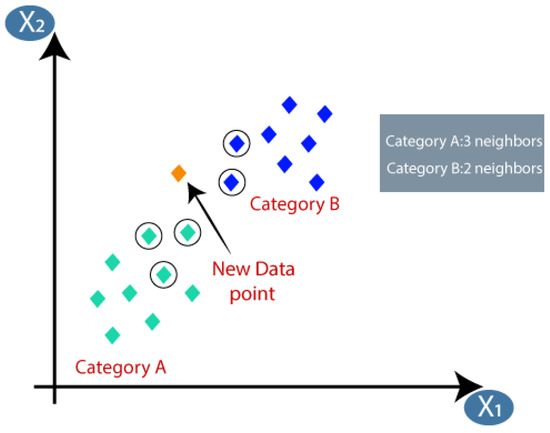
\includegraphics[width=0.9\linewidth]{images/image11.jpeg}
    \end{center}
\end{figure}

L'algoritmo k-nearest neighbors, noto anche come KNN o k-NN, è un classificatore di apprendimento supervisionato non parametrico.

Esso sfrutta la prossimità per effettuare classificazioni o previsioni sul raggruppamento di un singolo punto dati. 

Sebbene possa essere utilizzato per problemi di regressione o classificazione, viene generalmente impiegato in quanto algoritmo di classificazione, basandosi sul presupposto che dati simili, se analizzati o rappresentati nella giusta maniera, possono essere trovati l'uno vicino all'altro.

Per i problemi di classificazione un'etichetta di classe viene assegnata sulla base di un voto a maggioranza(ad es. viene utilizzata l'etichetta più frequentemente rappresentata attorno a un determinato punto dati).

I problemi di regressione utilizzano un concetto simile al problema di classificazione; in questo caso però viene presa la media dei k elementi vicini più vicini per effettuare una previsione su una classificazione. 

Qui, ciò che si discosta notevolmente, è il fatto che la classificazione viene utilizzata per i valori discreti, mentre la regressione viene utilizzata per quelli continui. 

Tuttavia, prima di poter effettuare una classificazione, è necessario definire il concetto di distanza. 

La distanza euclidea, altra metrica di distanza popolare, misura il valore assoluto tra due punti.

Vale la pena notare che l'algoritmo KNN fa anche parte di una famiglia di modelli di "apprendimento pigro", il che significa che memorizza solo un set di dati di addestramento nella fase di addestramento. 

Perviene quindi che tutto il calcolo avvenga quando si compie una classificazione o una previsione. 

Poiché fa ampiamente affidamento sulla memoria per archiviare tutti i suoi dati di addestramento, viene anche definito metodo di apprendimento basato su istanze o basato sulla memoria.

Le idee iniziali sul modello KNN sono attribuite a Evelyn Fix e Joseph Hodges in questo articolo [TODO trova articolo] del 1951, mentre Thomas Cover ne amplia il concetto nella sua ricerca, “Nearest Neighbor Pattern Classification.” [TODO trova articolo] 

Pur non riscuotendo un tale successo come in precedenza, è ancora uno dei primi algoritmi che si affronta nello studio della data science per la sua semplicità ed accuratezza. 

Tuttavia, al crescere di un set di dati KNN diventa sempre più inefficiente, compromettendo le prestazioni del modello. 

Viene riscontrato il suo impiego per semplici sistemi di raccomandazione, riconoscimento di modelli, data mining, previsioni dei mercati finanziari, rilevamento delle intrusioni e altro ancora. 

\subsubsection{Calcolare il KNN: metriche di distanza}
Ricapitolando, l'obiettivo dell'algoritmo k-nearest neighbor è identificare i vicini più prossimi di un dato punto di query, in modo da poter assegnare un'etichetta di classe a quel punto. 

Per determinare quali punti dati sono più attigui ad un determinato punto di query, sarà necessario calcolare la distanza tra il punto di interrogazione e gli altri punti dati. 

Le metriche di distanza aiutano a formare confini decisionali che suddividono i punti di query in regioni diverse. 

Sebbene sussistano diverse misure di distanza, tra cui è possibile scegliere, l’articolo sul sito di IBM tratta esclusivamente quelle a seguire:
\begin{itemize}
    \item Distanza euclidea (p=2): la misura della distanza più comunemente adottata; essa è limitata ai vettori con valori reali. 
    
    Utilizzando la formula seguente traccia una linea retta tra il punto di query e l'altro punto che si vuole misurare.
    \begin{figure}
        \begin{center}    
            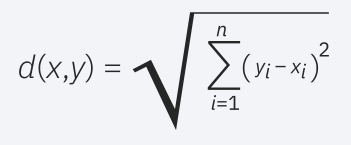
\includegraphics[width=0.45\linewidth]{images/image12.png}
        \end{center}
    \end{figure}
    \item Distanza di Manhattan (p=1): un'altra metrica di distanza particolarmente nota che si propone di misurare il valore assoluto tra due punti. 
    
    È anche riconosciuta come distanza del taxi o distanza del blocco cittadino, poiché è comunemente visualizzata con una griglia che illustra come si potrebbe percorrere il tragitto da un indirizzo all'altro attraverso le strade della città.
    \begin{figure}
        \begin{center}    
            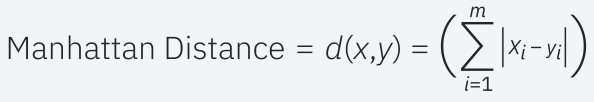
\includegraphics[width=0.45\linewidth]{images/image13.png}
        \end{center}
    \end{figure}
    \item Distanza di Minkowski: questa misura della distanza è la forma generalizzata delle metriche di distanza euclidea e di Manhattan. Il parametro, p, nella formula seguente, consente la creazione di altre metriche di distanza.    
    
    La distanza Euclidea è rappresentata da questa formula quando p è uguale a due e la distanza di Manhattan è indicata con p uguale a uno.

    \begin{figure}
        \begin{center}    
            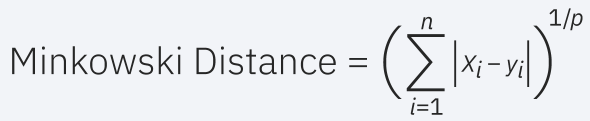
\includegraphics[width=0.45\linewidth]{images/image14.png}
        \end{center}
    \end{figure}

    \item Distanza di Hamming: questa tecnica viene utilizzata tipicamente con vettori booleani o stringa, identificando i punti in cui i vettori non trovano corrispondenza. 
    
    Di conseguenza, è stata anche definita metrica di sovrapposizione.
    \begin{figure}
        \begin{center}    
            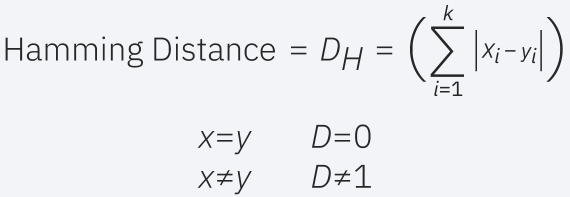
\includegraphics[width=0.45\linewidth]{images/image15.png}
        \end{center}
    \end{figure}
\end{itemize}

Ad esempio, se avessi le seguenti stringhe, la distanza di Hamming sarebbe due poiché solo due dei valori differiscono.

\begin{figure}
    \begin{center}    
        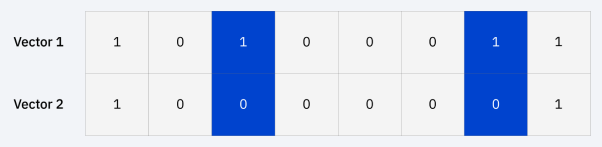
\includegraphics[width=0.8\linewidth]{images/image16.png}
    \end{center}
\end{figure}

\subsubsection{Calcolare KNN: definizione di k}
Il valore k nell'algoritmo k-NN definisce quanti vicini verranno controllati per determinare la classificazione di un punto di query specifico. 

Di fatti, se k=1, l'istanza verrà assegnata alla stessa classe del suo singolo neighbors più vicino. 

Definire k può essere un atto di bilanciamento, in quanto valori diversi possono portare a overfitting o underfitting. 

Valori inferiori a k possono essere caratterizzati da una variabilità elevata ma una bassa distorsione, mentre valori maggiori di k possono portare a una distorsione elevata e una variabilità inferiore. 

La scelta di k dipenderà in particolar modo dai dati di input, dal momento che i dati con più valori anomali o rumore probabilmente opereranno in modo più proficuo tanto più elevati sono i valori di k. 

In generale si consiglia di adoperare un numero dispari per k, col fine di evitare pareggi nella classificazione.

\subsubsection{Applicazioni di k-NN nell'apprendimento automatico}
L'algoritmo k-NN è stato utilizzato all'interno di una varietà di applicazioni, in maggior misura all'interno della classificazione. Alcuni di questi casi d'uso includono:
\begin{itemize}
\item Pre-elaborazione dei dati: poichè i dataset presentano spesso valori mancanti, l'algoritmo KNN può stimare tali valori in un processo noto come imputazione dei dati mancanti.
\item Recommender systems: adoperando i dati del flusso di clic dai siti web, l'algoritmo KNN è stato utilizzato per fornire consigli automatici agli utenti su contenuti aggiuntivi. Da tale ricerca emerge che un utente è assegnato a un particolare gruppo e, sulla base del comportamento di quest'ultimo, riceve un consiglio. Tuttavia, dati i problemi di scalabilità con KNN, questo approccio potrebbe non risultare ottimale in caso di impiego di dataset più grandi.
\item Finanza: è stato utilizzato anche in una varietà di casi di utilizzo finanziari ed economici. Ipoteticamente, un articolo mostra in che modo l'utilizzo di KNN sui dati di credito può aiutare le banche nella valutazione dei rischi su un prestito a un'organizzazione o a un individuo. Viene quindi sfruttato per determinare l'affidabilità creditizia del richiedente di tale prestito. Un altro articolo ne sottolinea l'uso nelle previsioni del mercato azionario, nei tassi di cambio, nel trading di fetures e nelle analisi sul riciclaggio di denaro.
\item Assistenza sanitaria: KNN ha riscontrato applicazioni anche nel settore dell'assistenza sanitaria, effettuando previsioni sul rischio di infarto e cancro alla prostata. L'algoritmo funziona calcolando le espressioni geniche più probabili.
\item Riconoscimento dei pattern: KNN ha anche aiutato a identificare i pattern, come nel testo e nella classificazione digitale. Ciò è stato particolarmente utile per identificare i numeri scritti a mano in cui ci si potrebbe imbattere su moduli o buste postali.
\end{itemize}
\subsubsection{Vantaggi e svantaggi dell'algoritmo KNN}
K-NN possiede i suoi punti di forza e di debolezza. A seconda del progetto e dell'applicazione, potrebbe rivelarsi o meno la scelta giusta.
\begin{itemize}
\item Vantaggi
\begin{itemize}
\item Facile da implementare: data la semplicità e l'accuratezza dell'algoritmo, è uno dei primi classificatori che un data scientist alle prime armi apprenderà.
\item Si adatta facilmente all'aggiunta di nuovi campioni di addestramento, l'algoritmo si adatta per tenere conto di eventuali nuovi dati, a fronte dell'archivio di tutti i dati di addestramento in memoria.
\item Pochi iperparametri: KNN necessita solo di un valore k e una metrica di distanza, il che, a confronto con altri algoritmi di machine learning, è minore in quantità.
\end{itemize}
\item Svantaggi
\begin{itemize}
\item Non è provvisto di una buona scalabilità: essendo KNN un algoritmo cosiddetto pigro, occupa più memoria e spazio di storage dei dati rispetto ad altri classificatori.
Sebbene diverse strutture di dati ,come Ball-Tree, siano state create per affrontare le inefficienze computazionali, un classificatore diverso potrebbe dimostrarsi ideale.
\item Maledizione della dimensionalità: l'algoritmo tende a cadere vittima della “maledizione della dimensionalità”; ciò significa che non ricopre adeguatamente il proprio ruolo con input di dati ad alta dimensionalità.
Questo è a volte indicato anche come il fenomeno del picco, nel quale, dopo che l'algoritmo raggiunge l'ottimale numero di funzioni, le funzioni aggiuntive aumentano la quantità di errori di classificazione, soprattutto quando la dimensione del campione è inferiore.
\item Propensione al sovradimensionamento dei dati: a causa della "maledizione della dimensionalità", KNN è anche più propenso al sovradimensionamento dei dati.
Sebbene le tecniche di selezione delle caratteristiche e di riduzione della dimensionalità vengano sfruttate per evitare che ciò accada, il valore di k può inevitabilmente influire sul comportamento del modello.
Valori più bassi di k possono sovra-alimentare i dati, mentre valori più alti di k tendono a "smussare" i valori di previsione, poiché si sta attuando la media dei valori su un'area o un neighborhood più grande.
Tuttavia, se il valore di k è troppo alto, può essere inferiore ai dati.
\end{itemize}
\end{itemize}

\subsection{Naive Bayes Classifier}
[da https://towardsdatascience.com/naive-bayes-classifier-81d512f50a7c]
Un classificatore di Bayes è un modello di apprendimento automatico probabilistico utilizzato per compiti di classificazione. Il fulcro del classificatore si basa sul teorema di Bayes.


\subsubsection{Teorema di Bayes}
Utilizzando il teorema di Bayes, possiamo trovare la probabilità che A accada, conseguentemente all’avvenimento di B. Qui, B è la prova e A è l'ipotesi. 

L'assunzione alla base del teorema è che i predittori e le caratteristiche siano indipendenti: in altre parole, la presenza di una particolare caratteristica non influisce sull'altra.
\begin{figure}
    \begin{center}    
        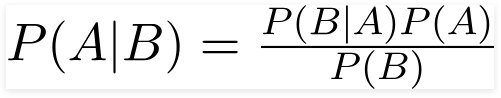
\includegraphics[width=0.9\linewidth]{images/image17.png}
    \end{center}
\end{figure}
Volendo offrire un esempio al fine di una migliore comprensione, consideriamo il problema di giocare a golf.  Il dataset è rappresentato come segue.
\begin{figure}
    \begin{center}    
        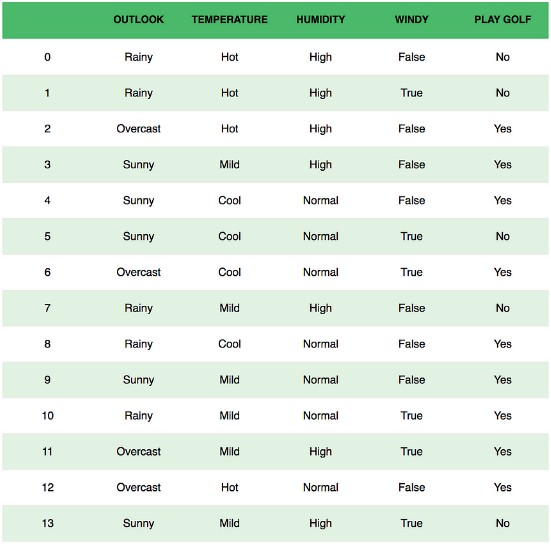
\includegraphics[width=0.9\linewidth]{images/image18.jpeg}
    \end{center}
\end{figure}
Classifichiamo se la giornata si configura adatta per una partita di golf, basandoci sugli attributi di tale giornata. Le colonne rappresentano questi attributi, mentre le righe rappresentano le singole voci.

Prendendo a campione la prima riga del dataset, possiamo osservare che non è adatta per giocare a golf se il cielo è nuvoloso, la temperatura è calda, l'umidità è alta e non c'è vento. Qui facciamo due assunzioni: 

come già detto, consideriamo che questi predittori siano indipendenti (ovvero, se la temperatura è calda, non significa necessariamente che l'umidità sia alta). Un'altra assunzione fatta qui è che tutti i predittori abbiano un effetto uguale sul risultato. Cioè, il fatto che ci sia vento non ha una maggiore importanza nella  decisione di giocare a golf o meno. 

Rifacendosi al secondo esempio, il teorema di Bayes può essere quindi riscritto come segue:

\begin{figure}
    \begin{center}    
        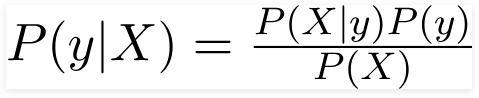
\includegraphics[width=0.9\linewidth]{images/image19.png}
    \end{center}
\end{figure}
La variabile y è la variabile di classe (giocare a golf), la quale rappresenta quanto sia adatta la giornata o meno per giocare a golf. La variabile X rappresenta i parametri/caratteristiche.


X è dato come segue:
\begin{figure}
    \begin{center}    
        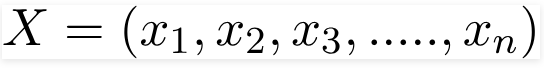
\includegraphics[width=0.9\linewidth]{images/image20.png}
    \end{center}
\end{figure}
Qui x1, x2... xn raffigurano le caratteristiche, cioè possono essere mappati su cielo, temperatura, umidità e vento. Sostituendo X ed espandendo utilizzando la regola della catena otteniamo:
\begin{figure}
    \begin{center}    
        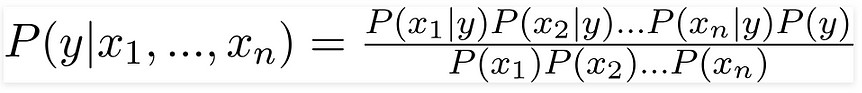
\includegraphics[width=0.9\linewidth]{images/image21.jpeg}
    \end{center}
\end{figure}
Ora è possibile ottenere i valori per ognuno guardando il dataset e sostituendoli nell'equazione. Per tutte le voci nel dataset, il denominatore non cambia, rimane statico. Pertanto, il denominatore può essere rimosso e può essere introdotta una proporzionalità.

\begin{figure}
    \begin{center}    
        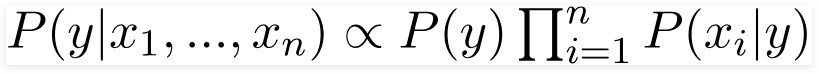
\includegraphics[width=0.9\linewidth]{images/image22.jpeg}
    \end{center}
\end{figure}
Nel nostro caso, la variabile di classe (y) ha solo due risultati, sì o no. Potrebbero esserci casi in cui la classificazione potrebbe rivelarsi multivariata. Pertanto, sarà necessario trovare la classe y con la massima probabilità.

\begin{figure}
    \begin{center}    
        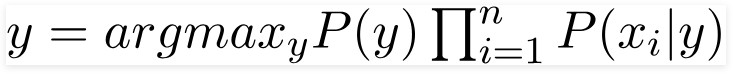
\includegraphics[width=0.9\linewidth]{images/image23.jpeg}
    \end{center}
\end{figure}
Utilizzando questa funzione ci è possibile ottenere la classe, dato il predittore.




\subsubsection{Tipi di Classificatori Bayesiani}
\begin{itemize}
\item Classificatore Bayesiano Multinomiale:
\begin{itemize}
\item Esso è principalmente utilizzato per problemi di classificazione dei documenti; ad esempio, se un documento appartiene alla categoria di sport, politica, tecnologia, ecc. Le caratteristiche/predittori impiegati dal classificatore saranno la frequenza delle parole presenti nel documento.
\end{itemize}
\item Classificatore Bayesiano di Bernoulli:
\begin{itemize}
\item Questo classificatore è simile al precedentemente citato, pur essendo i predittori variabili booleane. I parametri che usiamo per prevedere la variabile di classe assumono solo valori sì o no (se una parola compare nel testo o meno).
\end{itemize}
\item Classificatore Bayesiano Gaussiano:
\begin{itemize}
\item Quando i predittori assumono un valore continuo e non discreto, assumiamo che questi valori siano estratti da una distribuzione gaussiana.
\end{itemize}
\end{itemize}
Poiché il modo in cui i valori sono presenti nel dataset cambia, la formula per la probabilità condizionata cambia in questo caso,
\begin{figure}
    \begin{center}    
        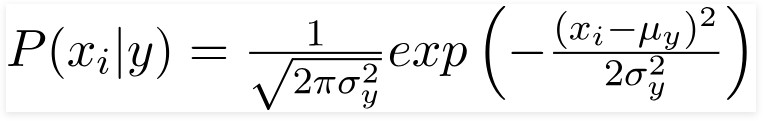
\includegraphics[width=0.9\linewidth]{images/image24.jpeg}
    \end{center}
\end{figure}

\subsubsection{Conclusione}
 
Gli algoritmi Bayesiani sono principalmente utilizzati nell'analisi del sentiment, nel filtraggio dello spam, nei reccomender systems, ecc. 

Sono veloci e facili da implementare, ma il loro più grande svantaggio è la necessità che i predittori siano indipendenti. 

Nella maggior parte dei casi reali, i predittori sono dipendenti, il che ostacola le prestazioni del classificatore.


\subsection{Support Vector Machine}
Il support vector machine è favorito maggiormente data la produzione di una significativa accuratezza mediante una minor potenza di calcolo. 

Il Support Vector Machine, abbreviato come SVM, può essere utilizzato sia per compiti di regressione che di classificazione. Tuttavia, viene ampiamente sfruttato negli obiettivi di classificazione.
\subsubsection{Cosa è il Support Vector Machine?}
L'obiettivo dell'algoritmo support vector machine è quello di trovare un iperpiano in uno spazio N- dimensionale (N - il numero di caratteristiche) che classifichi distintamente i punti dati.
\begin{figure}[h]
  \begin{minipage}[b]{0.45\linewidth}
    \centering
    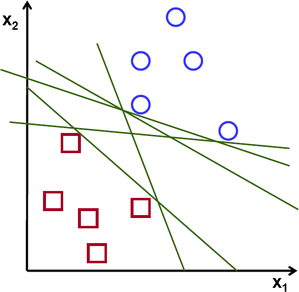
\includegraphics[width=\linewidth]{images/image25.png}
  \end{minipage}
  \begin{minipage}[b]{0.45\linewidth}
    \centering
    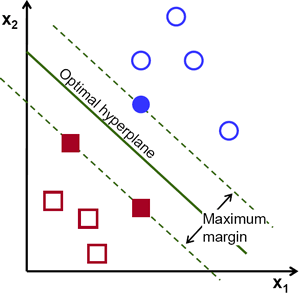
\includegraphics[width=\linewidth]{images/image26.png}
  \end{minipage}
\end{figure}
Per separare le due classi di punti dati sono presenti molti iperpiani possibili da cui poter scegliere. Il nostro obiettivo è trovare un piano che possegga il margine massimo, ovvero la massima distanza tra i punti dati di entrambe le classi. Massimizzare la distanza del margine fornisce un rinforzo in modo che i futuri punti dati possano essere classificati con maggiore fiducia.

Iperpiani e support vector
\begin{figure}
    \begin{center}    
        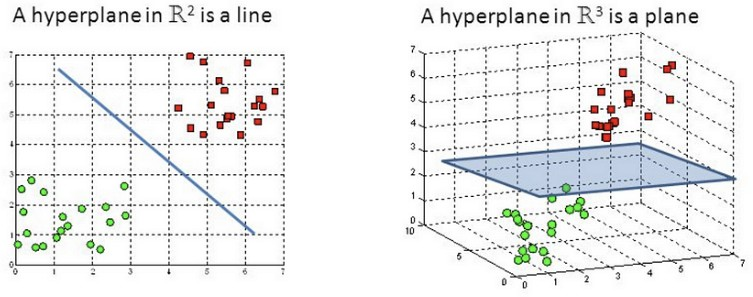
\includegraphics[width=0.9\linewidth]{images/image27.jpeg}
    \end{center}
\end{figure}
Gli iperpiani sono i confini decisionali che aiutano a classificare i punti dati. 

I punti dati che cadono su entrambi i lati dell'iperpiano possono essere attribuiti a diverse classi. 

Inoltre, la dimensione dell’iperpiano  dipende dal numero di caratteristiche. 

Se il numero di caratteristiche di input è 2, l'iperpiano è solo una linea. Se il numero di caratteristiche di input è 3, l'iperpiano diventa un piano bidimensionale. Diventa difficile immaginare quando il numero di caratteristiche supera 3.
\begin{figure}
    \begin{center}    
        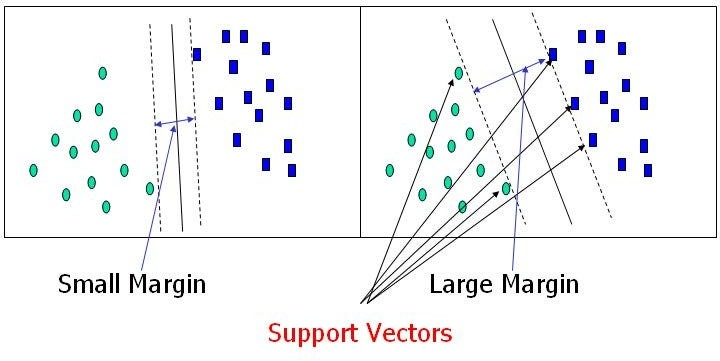
\includegraphics[width=0.9\linewidth]{images/image28.jpeg}
    \end{center}
\end{figure}
I support vector sono i punti dati più vicini all'iperpiano e influenzano la posizione e l'orientamento di quest’ultimo. Impiegando i support vector, massimizziamo il margine del classificatore. L’eliminazione  dei support vector cambierà la posizione dell'iperpiano. 

\subsubsection{Intuizione del grande margine}
Nella regressione logistica, prendiamo l'output della funzione lineare e normalizziamo il valore nell'intervallo  [0,1] utilizzando la funzione sigmoide. 

Se il valore normalizzato è maggiore di un valore soglia (0,5), gli assegniamo una etichetta 1, altrimenti gli assegniamo un'etichetta 0. 

Nell'SVM, prendiamo l'output della funzione lineare e, se quell'output è maggiore di 1, lo identifichiamo con una classe, mentre se l'output è -1, lo identifichiamo con un'altra classe. 

Poiché i valori della soglia sono cambiati in 1 e -1 nell'SVM, otteniamo questo intervallo ([-1,1]) che viene utilizzato come margine.


\subsubsection{Funzione di costo e aggiornamenti del gradiente}
Nell'algoritmo SVM, cerchiamo di massimizzare la distanza tra i punti dati e l'iperpiano. La funzione di perdita che ci aiuta a massimizzare la distanza è la hinge loss.
\begin{figure}[h]
  \begin{minipage}[b]{0.45\linewidth}
    \centering
    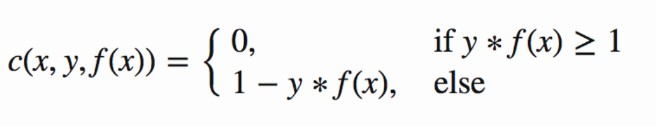
\includegraphics[width=\linewidth]{images/image29.jpeg}
  \end{minipage}
  \begin{minipage}[b]{0.45\linewidth}
    \centering
    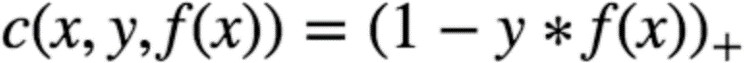
\includegraphics[width=\linewidth]{images/image30.jpeg}
  \end{minipage}
\end{figure}

Il costo è 0 se il valore previsto e il valore effettivo hanno lo stesso segno. In caso contrario, calcoliamo il valore di perdita. Aggiungiamo anche un parametro di regolarizzazione alla funzione di costo. L'obiettivo del
parametro di regolarizzazione è di bilanciare la massimizzazione della distanza con la perdita. 

Dopo aver aggiunto il parametro di regolarizzazione, la funzione di costo appare come segue.
\begin{figure}
    \begin{center}    
        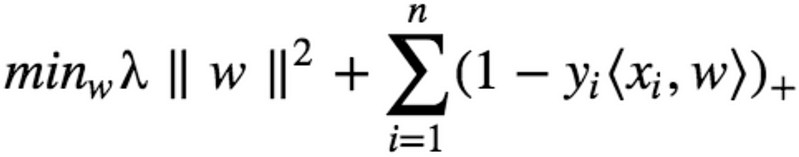
\includegraphics[width=0.9\linewidth]{images/image31.jpeg}
    \end{center}
\end{figure}
Ora che abbiamo ottenuto la funzione di perdita, utilizziamo le derivate parziali rispetto ai pesi per trovare i gradienti. 

Così facendo, possiamo aggiornare i pesi.
\begin{figure}
    \begin{center}    
        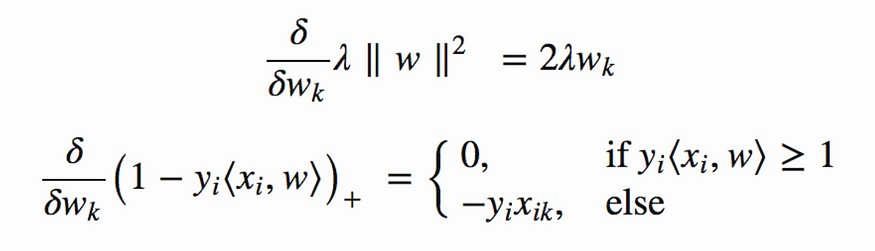
\includegraphics[width=0.9\linewidth]{images/image32.jpeg}
    \end{center}
\end{figure}
Quando non vi è alcuna errata classificazione, ovvero il nostro modello prevede correttamente la classe del nostro punto dati, sarà necessario aggiornare solo il gradiente dal parametro di regolarizzazione.
\begin{figure}
    \begin{center}    
        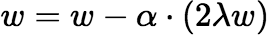
\includegraphics[width=0.9\linewidth]{images/image33.png}
    \end{center}
\end{figure}
Quando ci si trova di fronte ad una errata classificazione, ossia il nostro modello commette un errore sulla previsione della classe del nostro punto dati, includiamo la perdita insieme al parametro di regolarizzazione per eseguire l'aggiornamento del gradiente.


\begin{figure}
    \begin{center}    
        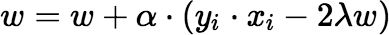
\includegraphics[width=0.9\linewidth]{images/image34.png}
    \end{center}
\end{figure}

\section{Random forest classifier}
Per effettuare delle predizioni sul dataset ho realizzato un classificatore random forest sul quale effettuare delle query, fornendogli i dati riguardanti le Action Units da nuove immagini, sempre attraverso la libreria py-feat.

Per la creazione del classificatore ho in primis letto il file csv contenente il dataset pre-elaborato (modifiche precedentemente trattate e sulle quali aggiungerò considerazioni, in quanto è risultato efficace applicarne ulteriori per migliorare la precisione del predittore creato), rimosso le colonne non necessarie e, infine, ho diviso il dataset in set di addestramento e di test usando la funzione train\_test\_split della libreria sklearn.model\_selection; tramite l’output di questo metodo ho ricavato i pandas’s dataframes Xtrain, Xtest, yTrain, yTest.

Questo è il metodo relativo:
\begin{minted}[bgcolor=bg]{python}
def getXtrainYTrainXtestYTest():
	pd.read_csv(join(dirname(
        abspath(__file__)), 
        "../final analysis/" + 
        "DAiSEE and student engagement dataset clean sampled.csv"
    ))
    y = df['label']
    X = df.drop(
        ["input","naturalLanguageDescription","label","numLabel"], 
        axis=1
    )
    
    Xtrain, Xtest, yTrain, yTest = train_test_split(
        X, 
        y, 
        test_size=0.2, 
        random_state=69
    )

    return Xtrain, yTrain 
\end{minted}
Una volta ottenuti questi dataset ho creato il classificatore utilizzando l’oggetto a disposizione fornito dalla libreria sklearn.ensable.

Il RandomForestClassifier viene generato con 100 alberi di decisione e viene addestrato con l’utilizzo dei due dataframe Xtrain e yTrain restituiti dalla funzione getXtrainYTrainXtestYTest().

Il metodo è il seguente:
\begin{minted}[bgcolor=bg]{python}
randomForestClassifier = RandomForestClassifier(n_estimators=100, verbose=True , random_state=42)
Xtrain, yTrain = getXtrainYTrainXtestYTest ()
randomForestClassifier.fit(Xtrain, yTrain)
return randomForestClassifier
\end{minted}

Eseguendo dei test attraverso il metodo \mintinline[bgcolor=bg]{python}{score(Xtest, yTest)} offerto dal random forest classifier generato dalla libreria sklearn.ensemble ho potuto calcolare l’accuracy del modello da me generato.

I risultati di questa analisi sono che il random forest classifier ottiene una precisione dell’82,3periodico% sul dataset di test generato nel metodo \mintinline[bgcolor=bg]{python}{getXtrainYTrainXtestYTest}

\begin{figure}
    \begin{center}    
        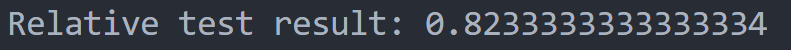
\includegraphics[width=0.9\linewidth]{images/image36.png}
    \end{center}
\end{figure}

Oltre alla produzione del classificatore viene anche generato un grafico per la visualizzazione dell’influenza di ognuna delle label sulla predizione che allego qui di seguito:

\begin{figure}
    \begin{center}    
        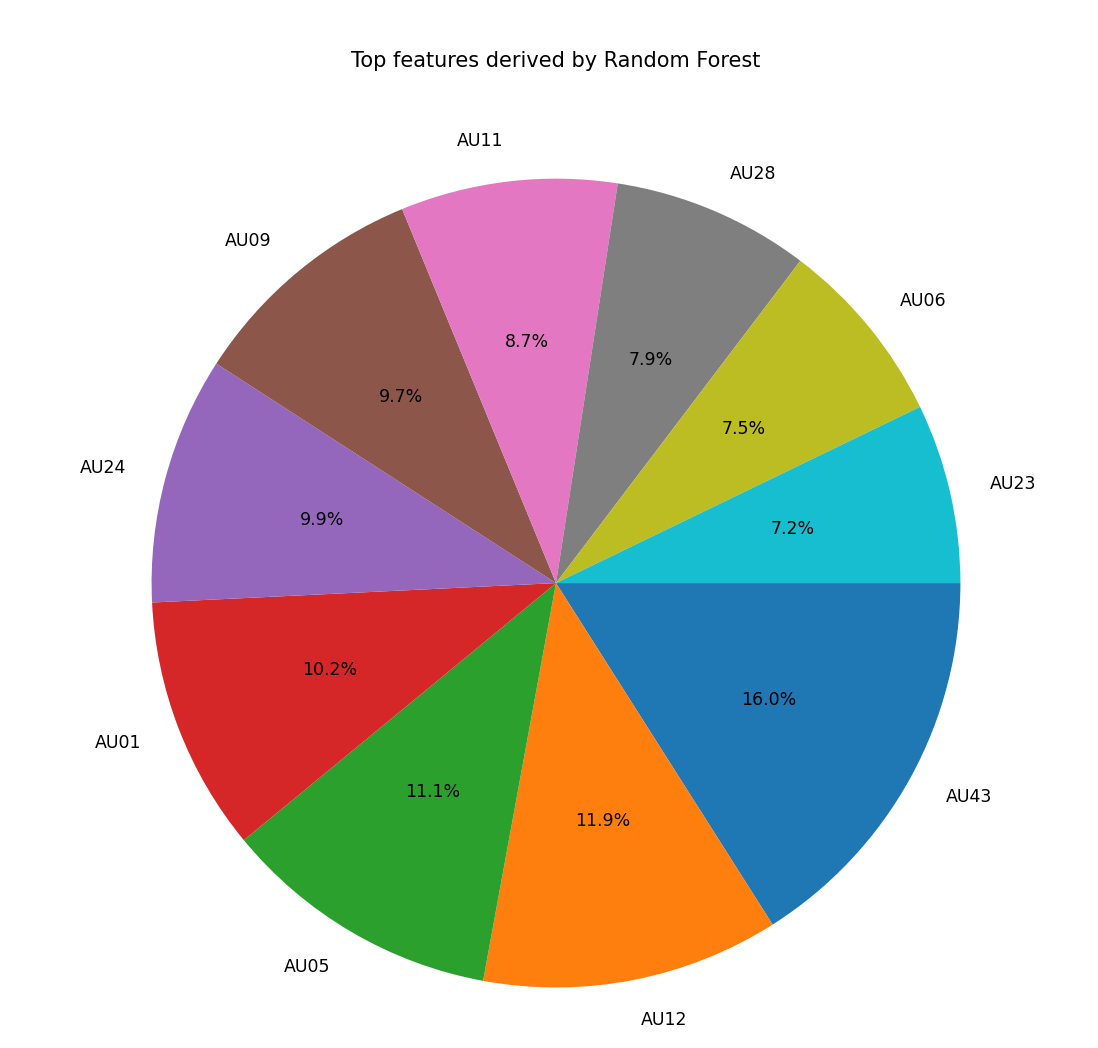
\includegraphics[width=0.9\linewidth]{images/image37.png}
    \end{center}
\end{figure}

Come è possibile constatare, quasi tutte le label influenzano la predizione in modo simile (in un range fra il 7,2% e l’11,9%) tranne per la AU43 (Eyes Closed) che, ovviamente, influenza largamente la predizione effettuata dal modello.

\section{K-nearest Neighbors Classifier}
Un ulteriore classificatore realizzato per effettuare predizioni sul dataset è il K-nearest Neighbors Classifier, attraverso il quale ho effettuato delle query fornendo i dati delle Action Units da nuove immagini.

Come per il random forest classifier, per la creazione del classificatore ho in primis letto il file csv contenente il dataset pre-elaborato, rimosso le colonne non necessarie e, infine, ho diviso il dataset in set di addestramento e di test usando la funzione train\_test\_split della libreria sklearn.model\_selection; tramite l’output di questo metodo ho ricavato i pandas’s dataframes Xtrain, Xtest, yTrain, yTest.

Il metodo sopracitato per l’estrazione di questi dataframe è lo stesso riportato in pochi paragrafi precedenti.

Una volta ottenuti questi dataset ho creato il classificatore utilizzando l’oggetto a disposizione fornito dalla libreria sklearn.neighbors.

Il K-nearest Neighbors Classifier viene creato impostando il parametro relativo al numero di elementi vicini da utilizzare settato a 1 e viene addestrato con l’utilizzo dei due dataframe Xtrain e yTrain restituiti dalla funzione getXtrainYTrainXtestYTest().

Il metodo è il seguente
\begin{minted}[bgcolor=bg]{python}
KnnClassifier = KNeighborsClassifier(n_neighbors=1)
Xtrain, yTrain = getXtrainYTrainXtestYTest ()
KnnClassifier.fit(Xtrain, yTrain)
return KnnClassifier
\end{minted}

Ho ritenuto opportuno valorizzare il campo con 1, in quanto è risultato il quantitativo necessario per non ottenere delle rilevazioni “ballerine” all’interno dell’interfaccia grafica da me realizzata e, allo stesso tempo, avere il miglior valore di accuracy possibile, calcolato come mostrato successivamente.

Ho poi eseguito il calcolo dell’accuratezza delle predizioni sul dataframe di test realizzato attraverso il seguente codice:
\begin{minted}[bgcolor=bg]{python}
from sklearn.metrics import accuracy_score
yPred = KnnClassifier.predict(Xtest)
accuracy = accuracy_score(yTest, yPred)
print("Accuracy: ", accuracy)
\end{minted}

ed ho ottenuto il seguente risultato:

\begin{figure}
    \begin{center}    
        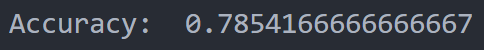
\includegraphics[width=0.9\linewidth]{images/image38.png}
    \end{center}
\end{figure}

Il classificatore K-nearest neighbors (KNN) determina l'importanza delle caratteristiche basandosi sulla loro influenza sulla metrica di distanza utilizzata per calcolare la vicinanza tra le istanze. 

Più le istanze sono vicine, più sono simili. Pertanto, le caratteristiche più importanti sono quelle che contribuiscono maggiormente al calcolo della distanza.

Un modo per visualizzare l'importanza delle caratteristiche per un classificatore KNN è quello di utilizzare una heatmap della matrice di correlazione a coppie delle caratteristiche. 

Le caratteristiche con correlazioni elevate avranno un impatto minore sul calcolo della distanza, mentre le caratteristiche non correlate riporteranno l' effetto contrario.

Il seguente codice viene utilizzato per disegnare una heatmap della matrice di correlazione delle caratteristiche:
\begin{minted}[bgcolor=bg]{python}
        def visualizeHeatMapCorrelationMatrix(Xtrain):
    corr = Xtrain.corr()
    sns.heatmap(corr, cmap='coolwarm')
    plt.show()
\end{minted}

Il colore di ogni quadrato nella heatmap rappresenta la correlazione tra due caratteristiche. 

Le caratteristiche altamente correlate saranno vicine tra loro nella heatmap, mentre le caratteristiche non correlate risulteranno distanti. 

\begin{figure}
    \begin{center}    
        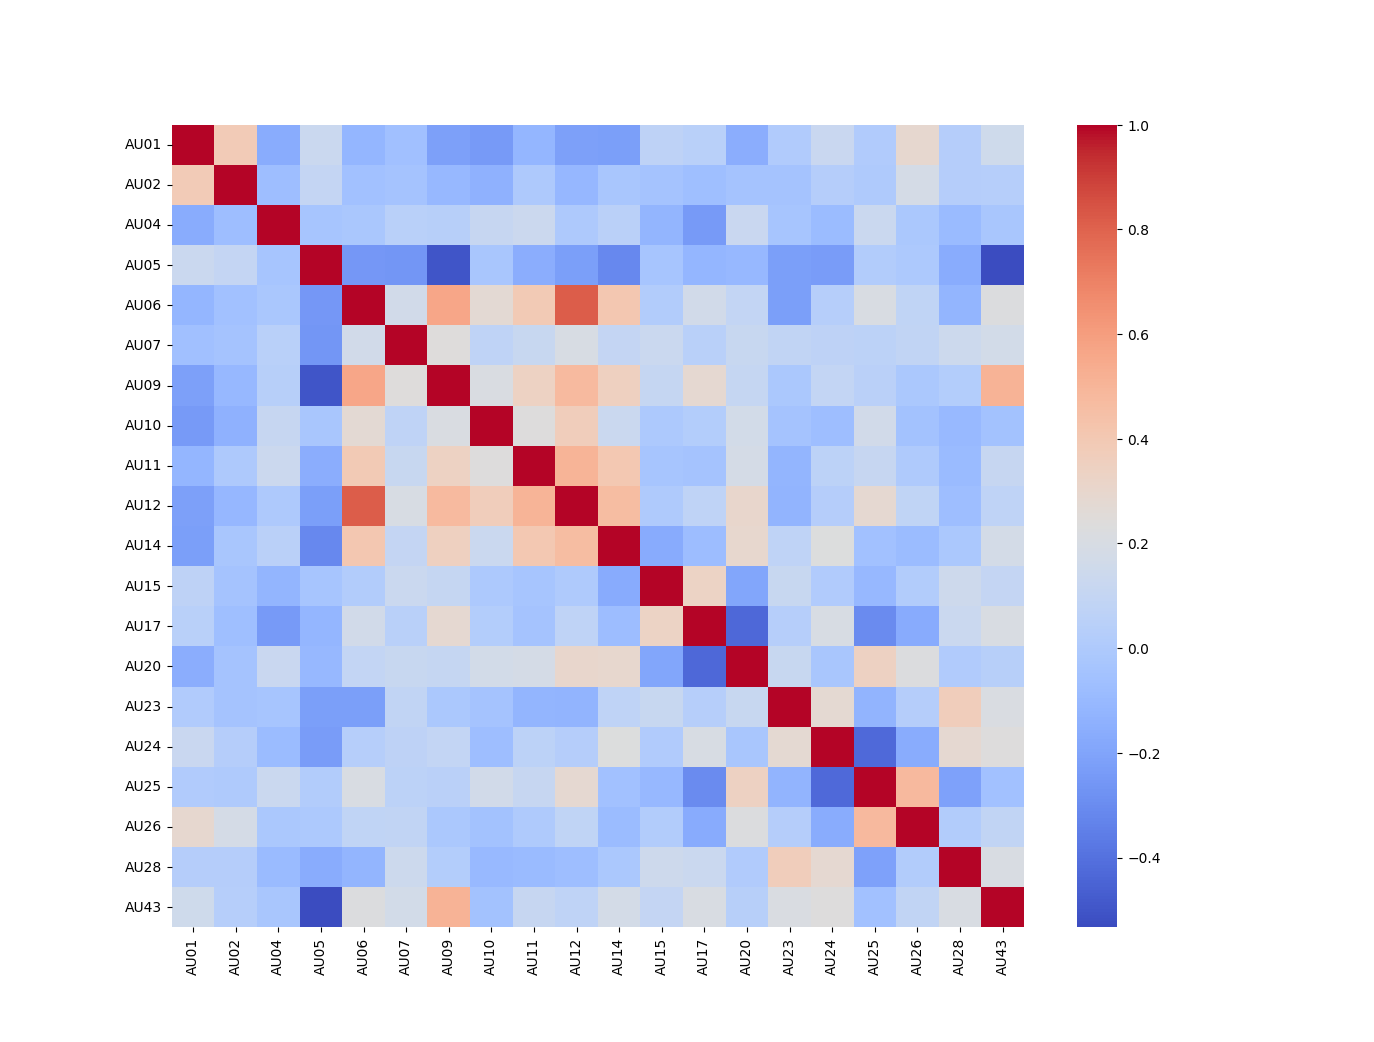
\includegraphics[width=0.9\linewidth]{images/image39.png}
    \end{center}
\end{figure}

Dalla heatmap riportata è possibile dedurre che, oltre all’ovvia correlazione di ogni Action Units a se stessa, ad esempio, la AU1 e la AU2 sono strettamente correlate, o ancora, AU12 e AU6 sono ancora più strettamente correlate, indi, influenzeranno particolarmente le predizioni risultanti.


\section{Support vector machine (SVM) Classifier}
Un altro classificatore adoperato per effettuare delle predizioni sul dataset è basato sull’algoritmo Support vector machine.

La modalità di realizzazione è molto simile a quella per i precedenti classificatori, con modalità di utilizzo identica al Random Forest classifier.

Viene sempre letto in memoria il dataset pre elaborato e resamplato, con successiva rimozione delle colonne non necessarie e viene suddiviso in set di addestramento e set di test.

L’oggetto che viene creato per effettuare le predizioni proviene sempre dalla libreria sklearn, in questo caso il modulo sklearn.svm e la sua relativa classe SVC.

Eseguendo dei test attraverso il metodo \mintinline[bgcolor=bg]
{python}{score(Xtest, yTest)} offerto dalla classe SVC ho potuto calcolare l’accuracy del modello da me generato:

\begin{figure}
    \begin{center}    
        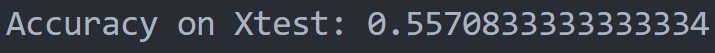
\includegraphics[width=0.9\linewidth]{images/image40.jpeg}
    \end{center}
\end{figure}

\section{Naive Bayes Classifier}
Un ulteriore classificatore di cui mi servo per effettuare delle predizioni sul dataset è basato sull’algoritmo Naive Bayes.

La modalità di realizzazione è molto simile a quella per i precedenti classificatori e la modalità di utilizzo è pari a quella del Random Forest classifier.

Viene sempre letto in memoria il dataset pre elaborato e resamplato, vengono rimosse le colonne non necessarie e viene suddiviso in set di addestramento e set di test.

L’oggetto che viene creato per effettuare le predizioni proviene sempre dalla libreria sklearn, in questo caso il modulo naive\_bayes e la sua relativa classe MultinomialNB.

Eseguendo dei test attraverso il metodo Eseguendo dei test attraverso il metodo \mintinline[bgcolor=bg]
{python}{score(Xtest, yTest)} offerto dalla classe MultinomialNB ho potuto calcolare l’accuracy del modello da me generato:

\begin{figure}
    \begin{center}    
        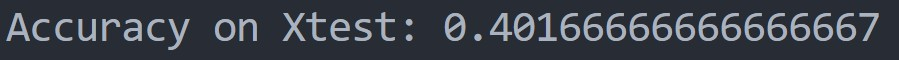
\includegraphics[width=0.9\linewidth]{images/image41.jpeg}
    \end{center}
\end{figure}

Il ~40\% di accuracy è il valore più alto che sono riuscito ad ottenere modificando i diversi valori presi in input dal costruttore di MultinomialNB.

\subsection{Quale modello predittivo risulta essere il migliore?}
Ho collezionato diverse metriche per valutare quale dei modelli predittivi sviluppati fosse il migliore: 
\subsection{Accuracy}
La metrica dell'accuracy è una delle metriche più comuni utilizzate per valutare la performance dei modelli predittivi. Essa misura la percentuale di predizioni corrette rispetto al numero totale di predizioni effettuate. Ad esempio, se un modello ha effettuato 100 predizioni e 80 di queste sono corrette, l'accuracy sarebbe del 80\%.

L'accuracy è una metrica particolarmente utile in caso, similmente al mio, di classi bilanciate. Ciò significa che il numero di esempi per ogni classe di output è simile. 

In questo contesto, può fornire una valutazione equilibrata della capacità del modello di predire entrambe le classi in modo corretto. 

Tuttavia, se le classi  non dovessero essere bilanciate, tale metrica potrebbe risultare fuorviante, dal momento che il modello potrebbe essere molto accurato nella predizione della classe maggioritaria ma non essere in grado di predire la classe di minoranza in modo corretto.

Un'altra considerazione importante quando si utilizza l'accuracy è il tipo di errore che si vuole minimizzare. Ad esempio, se il costo di un falso positivo è molto alto, allora un modello che massimizza l'accuracy potrebbe non essere la scelta migliore.

In formule, l'accuracy si calcola come:

\begin{figure}
    \begin{center}    
        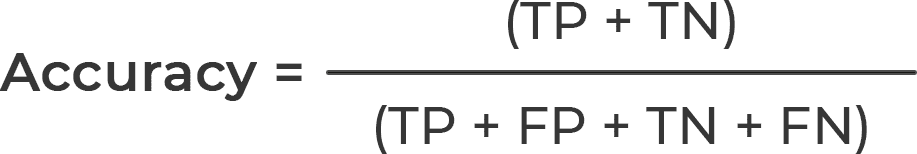
\includegraphics[width=0.9\linewidth]{images/image47.png}
    \end{center}
\end{figure}

dove TP indica il numero di veri positivi, TN indica il numero di veri negativi, FP indica il numero di falsi positivi e FN indica il numero di falsi negativi.

\subsection{Precision}
La metrica di precisione è una delle metriche più comuni utilizzate per valutare le prestazioni di un modello predittivo. La precisione è definita come la proporzione di predizioni corrette rispetto al totale delle predizioni fatte dal modello. In altre parole, la precisione misura quanto spesso il modello predittivo fornisce una risposta corretta rispetto al totale delle risposte fornite. È una misura di quanto preciso sia il modello nel predire le classi corrette.

Per calcolare la precisione di un modello predittivo occorre confrontare le predizioni effettuate dal modello con le etichette di classe corrette. La precisione è calcolata dividendo il numero di predizioni corrette per il totale delle predizioni effettuate dal modello. Ad esempio, se un modello predittivo ha effettuato 100 predizioni e 80 di queste predizioni sono corrette, la precisione del modello è del 80\%.

La metrica precision è definita come il rapporto tra il numero di veri positivi (TP) e il numero di tutti i casi predetti positivi (TP + FP). In altre parole, la precisione è la percentuale di volte in cui il modello ha predetto correttamente una classe positiva rispetto a tutte le volte in cui ha predetto quella classe.

Pur considerandosi utile, presenta alcune limitazioni. In particolare, la precisione non tiene conto dei falsi negativi, ovvero dei casi in cui il modello ha sbagliato a predire una classe positiva. Inoltre può essere influenzata dal numero di casi positivi e negativi presenti nel set di dati.

\begin{figure}
    \begin{center}    
        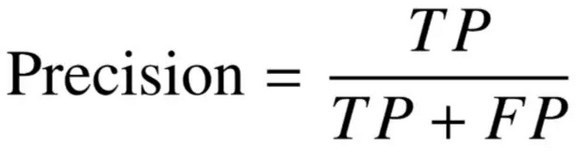
\includegraphics[width=0.9\linewidth]{images/image48.jpeg}
    \end{center}
\end{figure}

\subsection{Recall}
La metrica recall è una misura impiegata per la valutazione della capacità di un modello predittivo di identificare correttamente i veri positivi tra tutti i positivi effettivi. In altre parole, la recall comunica quanti dei casi positivi presenti in un insieme sono stati correttamente individuati dal modello.

Per calcolare la recall si divide il numero di veri positivi per la somma dei veri positivi e dei falsi negativi. In questo modo otteniamo una percentuale che fa emergere quanti dei casi positivi sono stati individuati dal modello.

Una delle principali ragioni dell’importanza di tale metrica è che ci permette di valutare la capacità del modello di individuare correttamente i casi positivi, anche se questo può comportare l’avere un alto numero di falsi positivi.

Un altro aspetto da considerare quando si utilizza la recall come metrica è che può essere influenzata dal bilanciamento delle classi. Ad esempio, se abbiamo un insieme di dati in cui la maggior parte dei casi sono negativi, potrebbe essere difficile ottenere una buona recall anche con un modello altamente performante.

Infine, è importante notare che la recall non ci comunica nulla sulla capacità del modello di classificare correttamente i casi negativi. Pertanto, è sempre importante considerare anche altre metriche come la precisione e l'accuratezza complessiva del modello quando si valutano le prestazioni complessive.

\begin{figure}
    \begin{center}    
        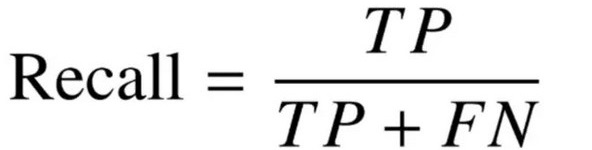
\includegraphics[width=0.9\linewidth]{images/image49.jpeg}
    \end{center}
\end{figure}

\subsection{Balanced Accuracy}
La metrica di Balanced Accuracy (o accuratezza bilanciata) è una misura di valutazione della performance di un modello predittivo che tiene conto della distribuzione bilanciata delle classi target all'interno del dataset di test. In altre parole, è una misura che considera l'accuratezza del modello in modo equilibrato per entrambe le classi target, evitando così di favorire una classe rispetto all'altra.

Per calcolare la metrica di Balanced Accuracy, si prende in considerazione la media aritmetica tra l'accuratezza della classe positiva (TPR) e quella della classe negativa (TNR), ovvero:
Balanced Accuracy = (TPR + TNR) / 2
 
Dove TPR (True Positive Rate) rappresenta la proporzione di veri positivi rispetto a tutti i casi positivi e TNR (True Negative Rate) rappresenta la proporzione di veri negativi rispetto a tutti i casi negativi.

In caso di dataset sbilanciati, in cui una classe target è più rappresentata dell'altra, la metrica di Balanced Accuracy risulta essere più informativa rispetto alla semplice accuratezza (Accuracy) in quanto fornisce una valutazione più equilibrata delle performance del modello per entrambe le classi target.

\begin{figure}
    \begin{center}    
        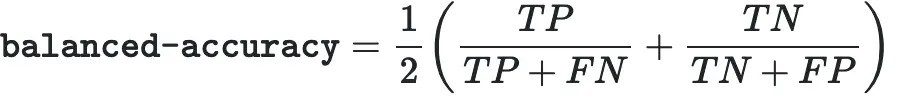
\includegraphics[width=0.9\linewidth]{images/image50.jpeg}
    \end{center}
\end{figure}

\subsection{Tabella dei risultati}
Tutte le metriche sono state calcolate a partire dai diversi modelli predittivi attraverso questo metodo:

\begin{minted}[bgcolor=bg]{python} 
def getModelScores(yTest, yPred):
from sklearn.metrics import accuracy_score, precision_score, recall_score, balanced_accuracy_score acc = accuracy_score(yTest, yPred)
prec = precision_score (yTest, yPred, average="weighted") recall = recall_score(yTest, yPred, average="weighted") balaAcc = balanced_accuracy_score(yTest, yPred)
return acc, prec, recall, balaAcc
\end{minted}
dove yTest è il dataframe estrapolato attraverso il metodo getXtrainYTrainXtestYTest precedentemente citato e yPred è la predizione effettuata sul dataframe Xtest, estratto sempre dallo stesso metodo, da parte del modello predittivo.

Ho opportunamente inserito tutte le metriche calcolate all’interno della tabella seguente per porre a confronto i modelli predittivi da me implementati:

\begin{table}[h]
\centering
\begin{tabular}{|l|c|c|c|c|}
\hline
& Accuracy & Precision & Recall & Balanced Accuracy \\
\hline
K-Nearest Neighbors & 78.54\% & 76.96\% & 78.54\% & 78.04\% \\
\hline
Random forest & 82.33\% & 82.05\% & 82.33\% & 81.97\% \\
\hline
Support vector machine & 55.70\% & 55.47\% & 55.70\% & 55.17\% \\
\hline
Naive bayes & 40.16\% & 35.55\% & 40.16\% & 39.49\% \\
\hline
\end{tabular}
\caption{Comparison of classification algorithms}
\label{tab:classification}
\end{table}

Come già evidenziato nel primo capitolo riguardante lo stato dell’arte, dalle analisi effettuate in \cite{FaceExpreRecoImgSeqTwoFoldRandomForestClass} l’algoritmo di random forest risulta essere il più affidabile per effettuare le previsioni su dataset di Action Units col fine di un rilevamento delle emozioni FACS e, come si evince dalla tabella sopra riportata, lo stesso è vero per gli stati d’animo (o moods) che vengono trattati nel mio caso di studio.